\documentclass[lettersize,journal]{IEEEtran}
\usepackage{amsmath,amsfonts}
\usepackage{algorithmic}
\usepackage{algorithm}
\usepackage{array}
\usepackage[caption=false,font=normalsize,labelfont=sf,textfont=sf]{subfig}
\usepackage{textcomp}
\usepackage{stfloats}
\usepackage{url}
\usepackage{verbatim}
\usepackage{graphicx}
\usepackage{cite}
\usepackage{xcolor}
\usepackage{xspace}
\usepackage{float} 
\usepackage[colorlinks,urlcolor=blue,linkcolor=blue,citecolor=blue]{hyperref}
\usepackage{orcidlink}
\usepackage{draftwatermark}

\SetWatermarkText{DRAFT}
\SetWatermarkColor[gray]{0.95}
\SetWatermarkFontSize{5cm}
\SetWatermarkAngle{45}
\SetWatermarkHorCenter{11cm}

\hyphenation{op-tical net-works semi-conduc-tor IEEE-Xplore}

\newcommand{\MATLAB}{\textsc{Matlab}\xspace}
\newcommand{\SIMULINK}{\textsc{Simulink}\xspace}

\def\BibTeX{{\rm B\kern-.05em{\sc i\kern-.025em b}\kern-.08em T\kern-.1667em\lower.7ex\hbox{E}\kern-.125emX}}

\begin{document}
	
	\title{Comparing the SFDR Performance of LUT size and DDS Spurious Improvement Algorithms}
	
	\author{Simon M. Burkhardt \IEEEmembership{Student Member,~IEEE} \textsuperscript{\large\orcidlink{0000-0003-4568-9780}}
		\thanks{Manuscript received Month xx, 2023.}
		\thanks{S. M. Burkhardt is with the University of Applied Sciences and Arts Northwestern Switzerland, Windisch, CH-5210 Switzerland (e-mail: simon.burkhardt@ fhnw.ch).}
	}
	
	% The paper headers
	\markboth{IEEE TRANSACTIONS ON MICROWAVE THEORY AND TECHNIQUES, ~VOL.~*, NO.~*, *~2023, ID: TMTT-2023-01-0078}
	{Burkhardt \MakeLowercase{\textit{et al.}} }
	
	%Note: There should no nonstandard abbreviations, acknowledgments of support, references or footnotes in in the abstract.}

\maketitle

		\begin{abstract}
	With the performance increase of high frequency digital to analog converters, digital synthesizers continue to replace traditional analog oscillator circuits. Traditional Direct Digital Synthesizers (DDS) use lookup tables to convert phase to sinusoidal amplitude. The phase truncation occurring in this architecture seriously limits the spectral performance of the generated signal in the form of spurs. This work uses MATLAB/Simulink to reproduce the frequency errors widely discussed in literature. The simulation framework is then used to apply various amplitude treatement algorithms to correct the signal and improve the spurious performance. Furthermore, the algorithms are compared against each other to find the best method in terms of spurious free dynamic range (SFDR), consumed hardware resources on FPGA and latency. The proposed design includes an 8 channel polyphase DDS with linear interpolation correction and an expected SFDR of below $-105$\,dBc.	
	\end{abstract}

% discretion; the only required sections are Introduction, Methods and 
% Procedures, Results, Conclusion, and References. Acknowledgements and 
% Appendices are encouraged but optional.)

\begin{IEEEkeywords}
	Direct Digital Synthesis, Bit True Simulation, Spurious Performance Analysis, High Frequency Signal Generation
\end{IEEEkeywords}

\section{INTRODUCTION}

\IEEEPARstart{U}{sing} digital signal processing to synthesize analog waveforms is a well established method generate a sinewaves of variable frequency. A commonly used architecture is that of the Direct Digital Synthesis (DDS). One major disadvantage of a DDS system is that a truncation of the phase accumulator needs to be implemented to keep the memory size of the sine look up table (LUT) reasonably small. This truncation leads to phase errors and inevitably truncation spurs in the spectral domain. Many signal processing algorithms have been proposed in the past. Their goal is to minimize truncation spurs while maintaining small LUT sizes.

However, there appears to be no general overview and comparison of the algorithms that anwers the following question quickly:
What combination of LUT size and correction algorithm do I need to achieve a signal with $x$ dB spurious free dynamic range?

This work aims to build a bit-true simulation model in Python to simulate the traditional DDS as well as several spurious correction algorithms in order to compare them in the spectral domain. Not only are the effects of phase truncation and quantization visible, but all the DSP calculations are performed using fixed point arithmetic. The example chosen are the DSP48E2 Slices available in Xilinx FPGA, capable of working with a minimum of 18 bits precision.





\subsection{Results}


\section{Conclusion}


\section*{Acknowledgment}


\begin{thebibliography}{00}
	\bibitem{tang_linar_int} S. Tang, C. Li and Y. Hou, ``Suppressing Method for Spur Caused by Amplitude Quantization in DDS,'' in IEEE Access, vol. 7, pp. 62344-62351, 2019, \url{https://doi.org/10.1109/ACCESS.2019.2915677}
	
	\bibitem{zang_taylor} J. Zhang, R. Zhang and Y. Dai, ``Design and FPGA implementation of DDS based on waveform compression and Taylor series,'' 2017 29th Chinese Control And Decision Conference (CCDC), Chongqing, China, 2017, pp. 1301-1306, \url{https://doi.org/10.1109/CCDC.2017.7978718}
	
	\bibitem{langolis_novel} J. M. P. Langlois and D. Al-Khalili, ``Novel approach to the design of direct digital frequency synthesizers based on linear interpolation,'' in IEEE Transactions on Circuits and Systems II: Analog and Digital Signal Processing, vol. 50, no. 9, pp. 567-578, Sept. 2003, \url{https://doi.org/10.1109/TCSII.2003.815020}


\end{thebibliography}

\begin{IEEEbiography}[{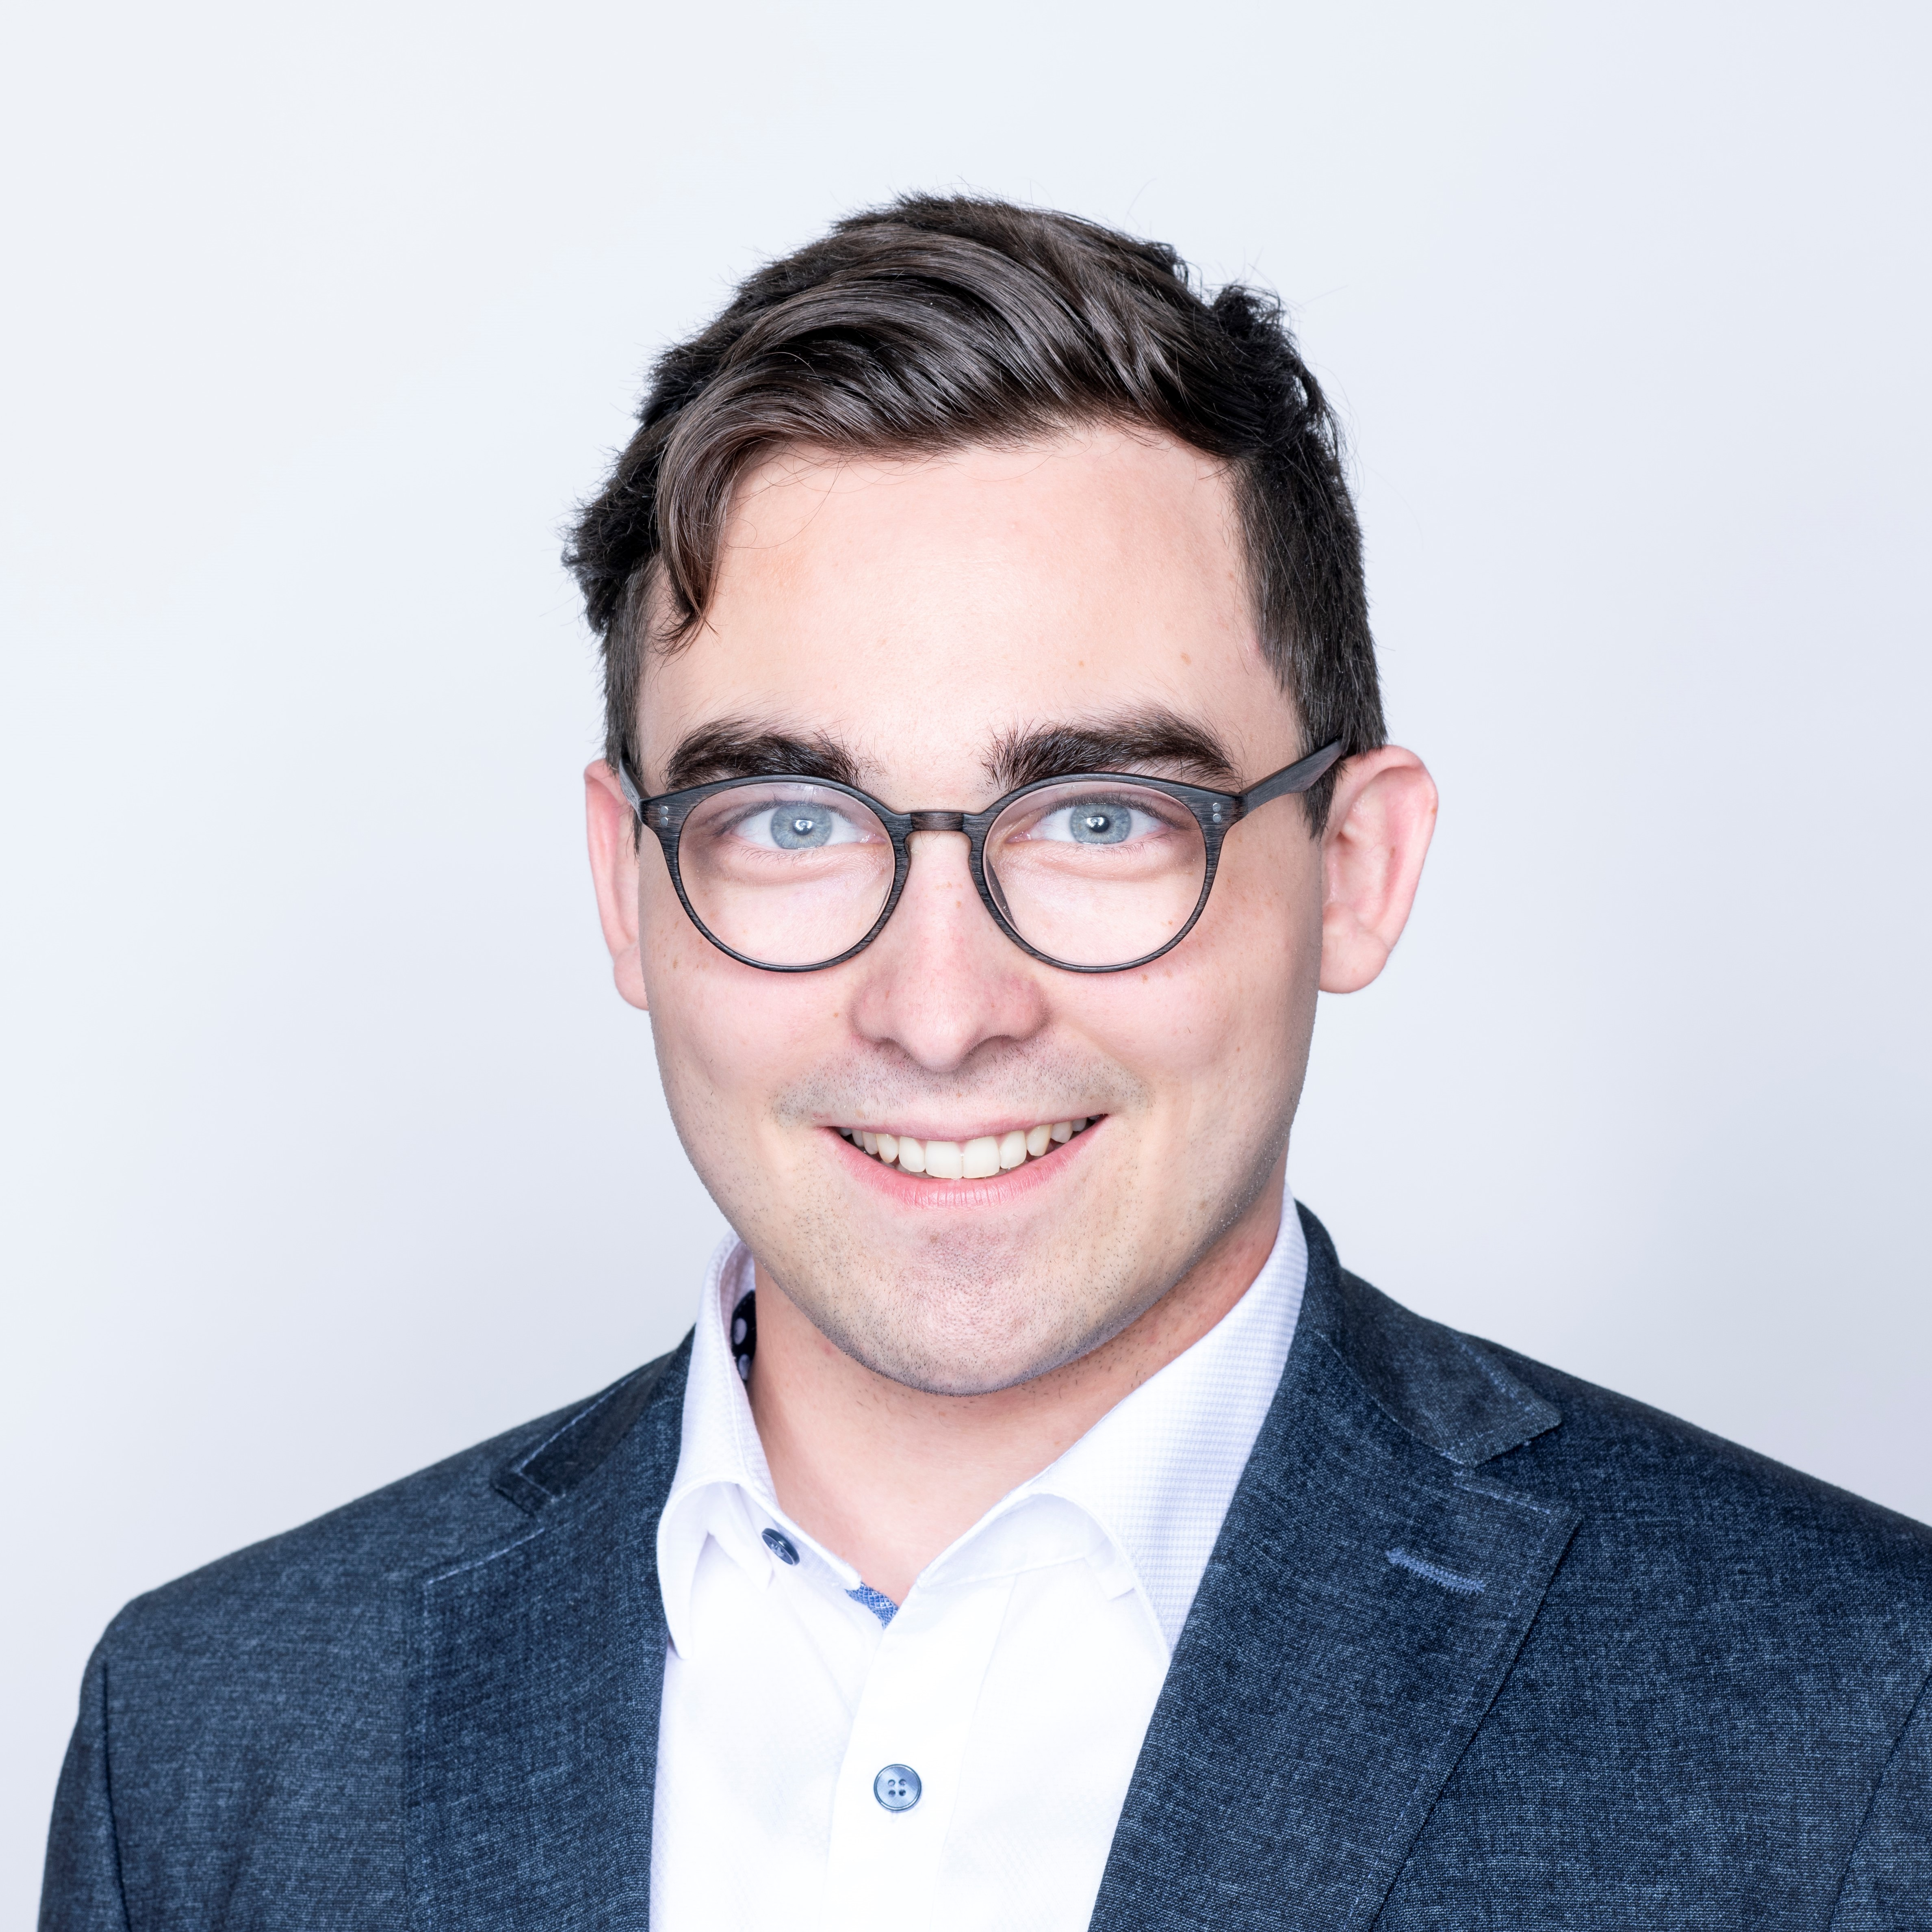
\includegraphics[width=1in,height=1.25in,clip,keepaspectratio]{figures/simon_quare.jpg}}]{Simon Martin Burkhardt}{\,}received the B.S. in electrical and information technologies in 2020 and is currently pursuing an M.S. degree in the same field, both at the Institute of Sensors and Electronics (ISE) at the University of Applied Sciences and Arts of Northwestern Switzerland (FHNW) in Windisch, Switzerland. There he is currently a research assistant for embedded systems.
His primary research interests are in embedded systems design, FPGA design and digital signal processing.
He is an IEEE student member since 2015.
Contact him at simon.burkhardt@fhnw.ch
\end{IEEEbiography}


\vfill

\end{document}
